% Chapter 1

\chapter{Introducción general} % Main chapter title

\label{Chapter1} % For referencing the chapter elsewhere, use \ref{Chapter1} 
\label{IntroGeneral}

%----------------------------------------------------------------------------------------

% Define some commands to keep the formatting separated from the content 
\newcommand{\keyword}[1]{\textbf{#1}}
\newcommand{\tabhead}[1]{\textbf{#1}}
\newcommand{\code}[1]{\texttt{#1}}
\newcommand{\file}[1]{\texttt{\bfseries#1}}
\newcommand{\option}[1]{\texttt{\itshape#1}}
\newcommand{\grados}{$^{\circ}$}

En este capítulo se realiza una introducción al protocolo Modbus y la vinculación con la internet de las cosas. Asimismo, se mencionan algunos sistemas en el mercado, y por último se explica la motivación, alcance y objetivos del presente trabajo.


%----------------------------------------------------------------------------------------

%\section{Introducción}

%----------------------------------------------------------------------------------------
\section{Comunicación Modbus y supervisión SCADA}

Gracias al desarrollo e innovación de nuevas tecnologías y a la automatización de procesos industriales a través del tiempo, se ha dado lugar a avances significativos que le han permitido a industrias implementar procesos de producción eficientes, seguros y competitivos.

Actualmente en el sector industrial es muy utilizado el PLC (\textit{Programmable Logic Controller}) \citep{WEBSITE:1} para controlar máquinas, líneas de producción y en general todo lo relacionado con el proceso propio de la industria, y para que esto sea posible, los equipos, sensores y actuadores deben comunicarse entre sí. Con este fin se utiliza, entre otros, el protocolo de comunicación Modbus  \citep{WEBSITE:2}, introducido por la empresa Modicon en 1979. 

Modbus permite conectar un dispositivo servidor con varios dispositivos clientes.  Existen dos versiones de implementación:
\begin{itemize}
	\item Interfaz serie (RS-232 y RS-485) llamada Modbus serie.
	\item Interfaz Ethernet llamada Modbus TCP.
\end{itemize}

%Modbus es un protocolo de mensajería de capa de aplicación, posicionado en el nivel 7 del modelo OSI \citep{WEBSITE:3}.  La comunicación está basada en un %protocolo de solicitud / respuesta,  donde es siempre iniciada por el servidor y,  por lo tanto, los clientes nunca transmitirán datos sin una solicitud previa.  


Modbus es un protocolo de mensajería de capa de aplicación, posicionado en el nivel 7 del modelo OSI \citep{WEBSITE:3}. Proporciona comunicación cliente / servidor entre dispositivos conectados en diferentes tipos de buses o redes. Es un protocolo de solicitud / respuesta en el cuál el servidor realiza consultas de datos a un cliente de la red.


Las solicitudes desde el nodo servidor a los clientes pueden ser realizados en dos modos:
\begin{itemize}
	\item Modo unicast: en este modo,  el servidor direcciona a un esclavo.
	\item Modo broadcast: en este modo, el servidor envía una solicitud a todos los esclavos simultáneamente, sin recibir respuesta.
\end{itemize}

Este protocolo permite comunicarse de manera sencilla con todo tipo de arquitecturas de red como puede observarse en la figura \ref{fig:red-modbus}, y además,  con el uso de \textit{gateways} se puede interactuar entre varios tipos de buses o redes.

\begin{figure}[htpb]
	\centering
	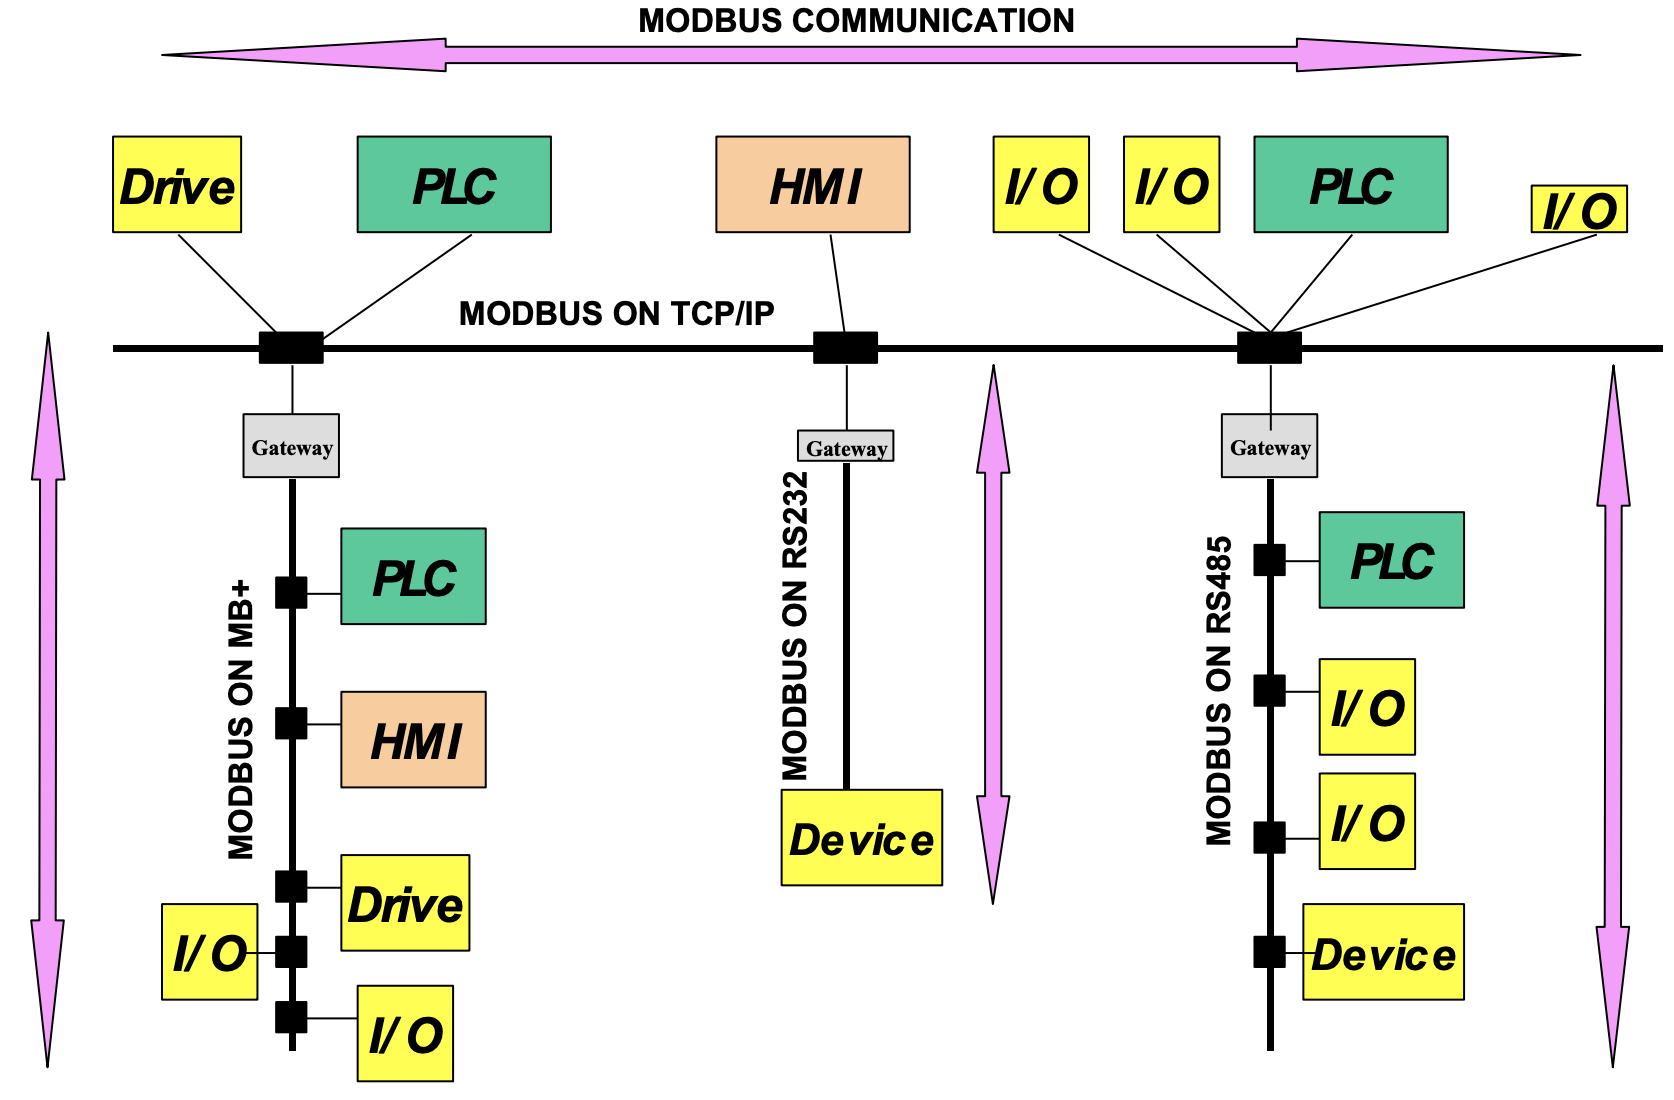
\includegraphics[scale=.48]{./Figures/red-modbus.png}
	\caption[Arquitectura de red Modbus.]{Ilustración de diferentes arquitecturas de red utilizando el protocolo Modbus\protect\footnotemark.}
	\label{fig:red-modbus}
\end{figure}

\footnotetext{\url{https://modbus.org/docs/Modbus_Application_Protocol_V1_1b3.pdf}}

Para la supervisión y control de un proceso industrial que utiliza Modbus como protocolo de comunicación,  se utilizan sistemas HMI (\textit{Human Machine Interface}) y hacen referencia a la manera que interactúa el humano con las diferentes máquinas que componen el sistema. 

Se trata de un sencillo panel que transmite órdenes, visualiza resultados de manera gráfica y obtiene visualización del estado del proceso o la máquina en tiempo real.  

A modo de ejemplo se pueden observar en la figura \ref{fig:hmi-siemens} diferentes modelos de HMI de la empresa Siemens. 

\begin{figure}[htpb]
	\centering
	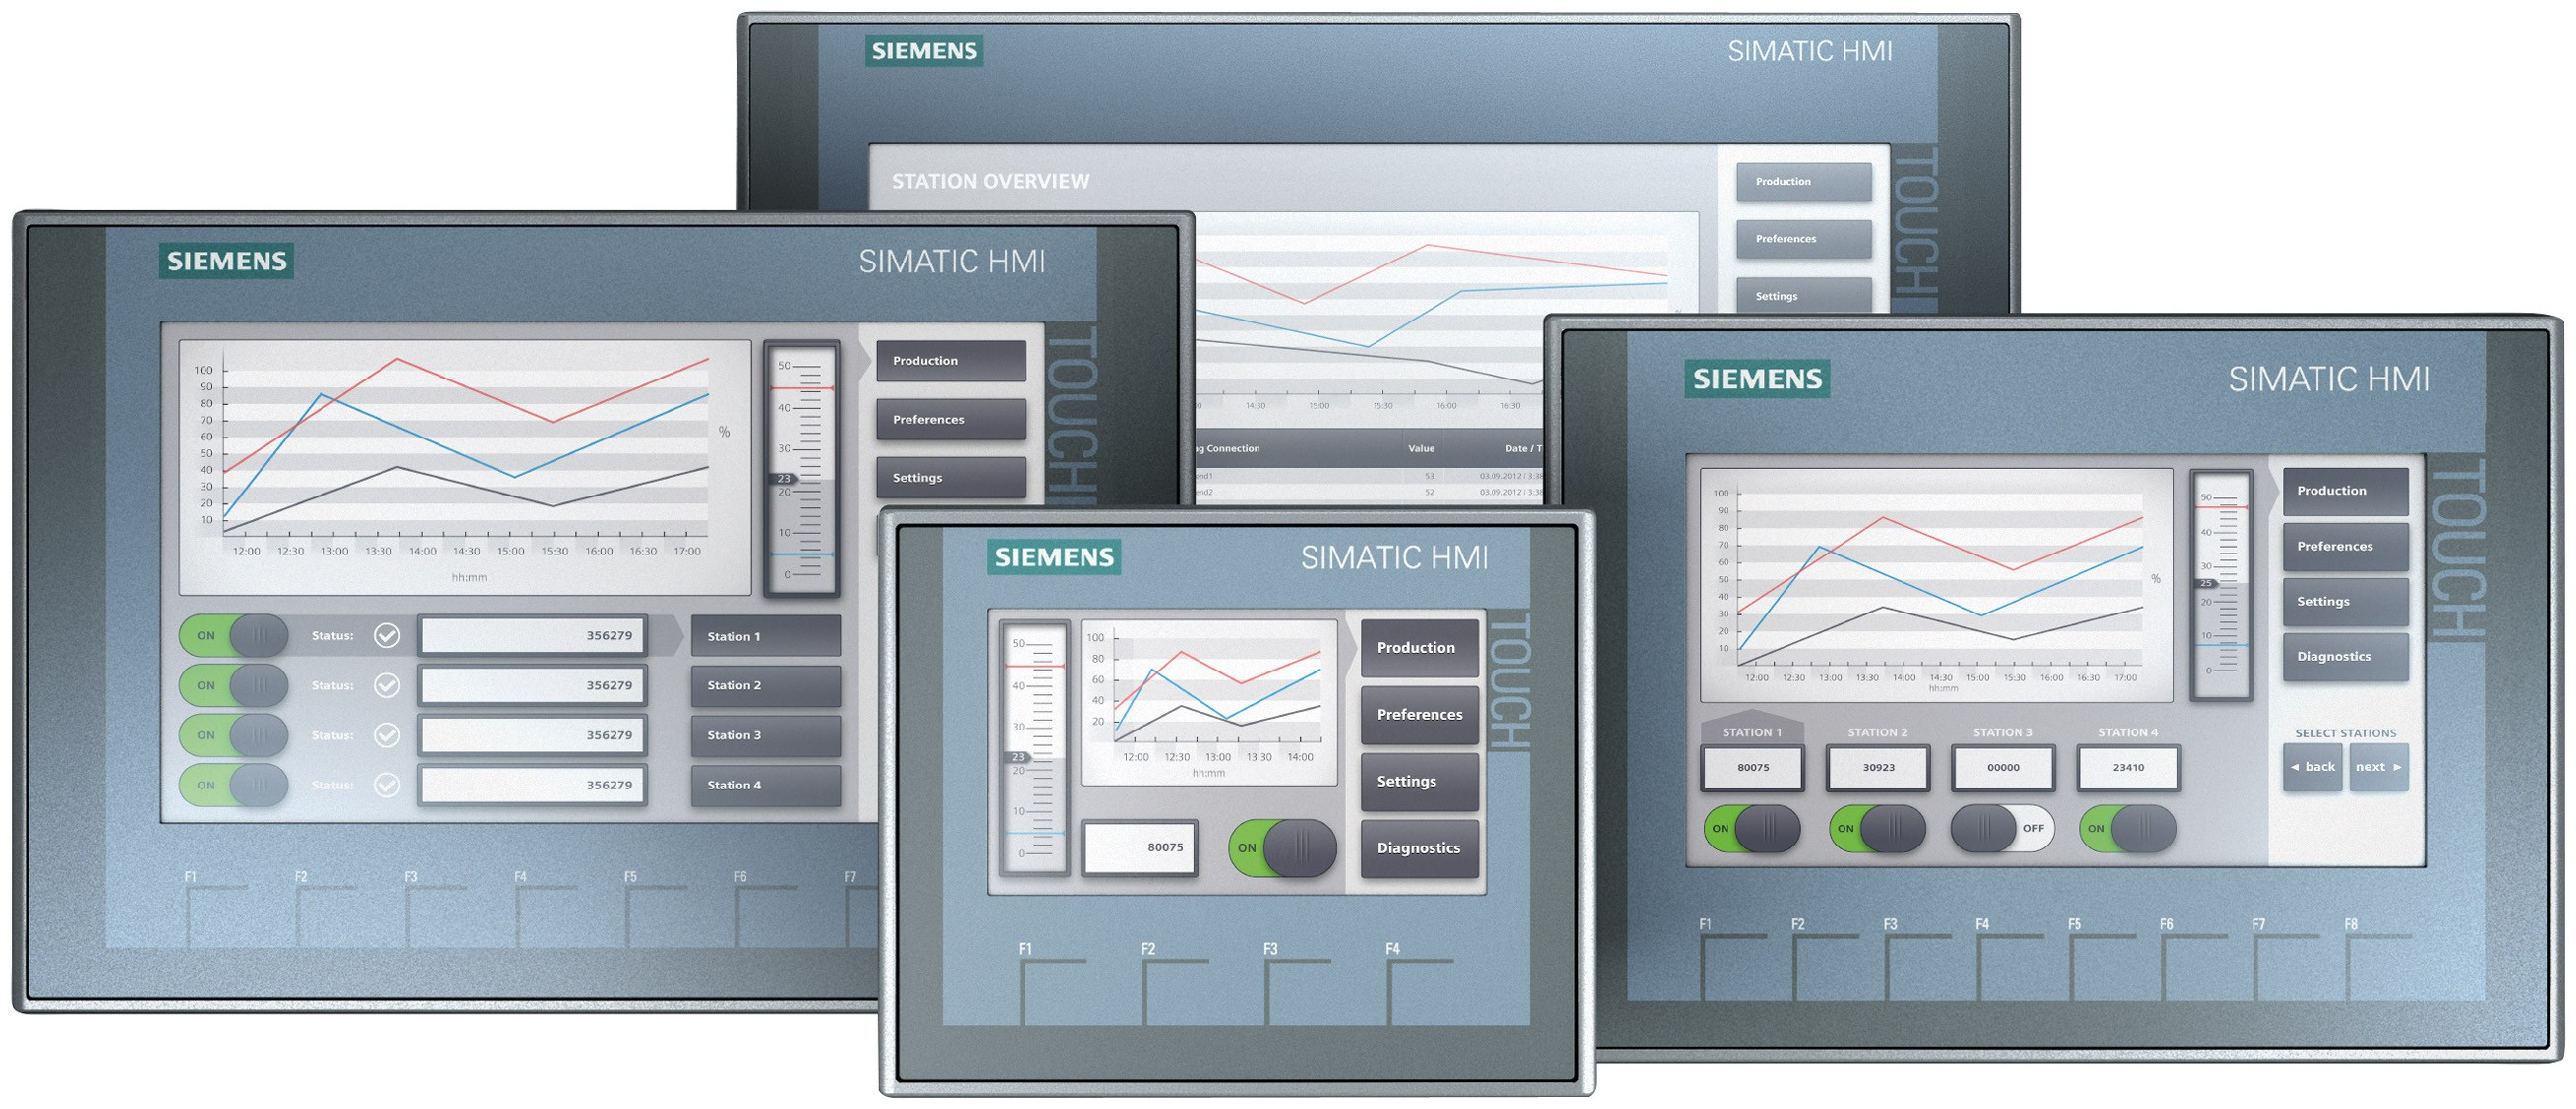
\includegraphics[scale=.10]{./Figures/hmi-ejemplos.jpg}
	\caption[Diferentes modelos de HMI de la empresa Siemens]{Diferentes modelos de HMI de la empresa Siemens\protect\footnotemark.}
	\label{fig:hmi-siemens}
\end{figure}

\footnotetext{\url{https://new.siemens.com/global/en/products/automation/simatic-hmi/panels/basic-panels.html}}

En un nivel superior de gestión del proceso industrial antes mencionado, se encuentra el sistema SCADA,  cuya palabra es un acrónimo que deriva del inglés  \textit{Supervisory Control And Data Acquisition} y su significado en español se traduce como Control Supervisor y Adquisición de Datos.

Los sistemas SCADA son programas de software que se utilizan para gestionar y controlar sistemas remotos o locales mediante el uso de una interfaz gráfica que comunica al usuario con el programa.  Cuentan con una estructura que parte de sus controladores lógicos programables (PLC) o unidades de terminal remotas (RTU)\citep{BOOK:1}, es decir, de microordenadores que se comunican con múltiples objetos, ya sean máquinas, dispositivos, sensores o HMI. Estos microordenadores después de comunicar, envían la información desde estos objetos a los ordenadores con el software SCADA.  

Por lo tanto, el sistema SCADA procesa, distribuye y muestra los datos, permitiendo a los operadores y otros trabajadores realizar un análisis para facilitar la toma de decisiones. Entre sus principales características, podemos destacar:

\begin{itemize}
	\item Supervisar remotamente las instalaciones y equipos.
	\item Monitorizar y controlar las operaciones en tiempo real.
	\item Procesar datos que hagan más fácil la toma de decisiones.
	\item Mostrar a través de imágenes dinámicas el comportamiento de los procesos.
	\item Arrojar señales de alarma (visuales o sonoras) frente a imprevistos.
\end{itemize}

En la figura \ref{fig:wincc-siemens} se puede observar la implementación de un sistema SCADA realizado con el software WINCC \citep{WEBSITE:4}  de la empresa Siemens para el monitoreo y gestión de energía eléctrica. 

\begin{figure}[htpb]
	\centering
	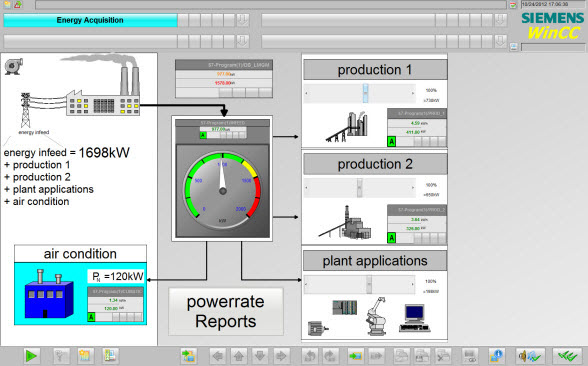
\includegraphics[scale=.7]{./Figures/wincc-siemens.jpg}
	\caption[Implementación de sistema SCADA con WINCC]{Ejemplo de implementación de un sistema SCADA con el software WINCC de la empresa Siemens para monitoreo y gestión de energía eléctrica\protect\footnotemark.}
	\label{fig:wincc-siemens}
\end{figure}

\footnotetext{\url{https://support.industry.siemens.com/cs/document/65384955/gestión-de-energía}}

%----------------------------------------------------------------------------------------

%\section{IIoT}

%----------------------------------------------------------------------------------------
\section{Internet de las cosas}

Por lo general, el término Internet de las cosas (IoT) se refiere a escenarios en los que la conectividad de red y la capacidad de cómputo se extienden a objetos, sensores y artículos de uso diario que habitualmente no se consideran computadoras, permitiendo que estos dispositivos generen, intercambien y consuman datos con una mínima intervención humana.  

El concepto de combinar computadoras, sensores y redes para monitorear y controlar diferentes dispositivos ha existido durante décadas. Sin embargo, la reciente confluencia de diferentes tendencias del mercado tecnológico está permitiendo que la internet de las cosas esté cada vez más cerca de ser una realidad generalizada.   

Estas tendencias incluyen la conectividad omnipresente, la adopción generalizada de redes basadas en el protocolo IP \citep{WEBSITE:9}, la economía en la capacidad de cómputo, la minimización, los avances en el análisis de datos y el surgimiento de la computación en la nube.

Los beneficios que internet de las cosas ofrece tanto a empresas como a personas individuales son numerosos. Desde un punto de vista económico, permite a las empresas gestionar y controlar mejor sus procesos de forma remota y en tiempo real, aumentando su eficiencia y posibilitando la toma de mejores decisiones y acciones preventivas como el mantenimiento de la maquinaria o sistemas instalados. En definitiva, esto conlleva un ahorro de costos y tiempo para la organización. En el caso de individuos particulares, los beneficios se traducen en mejoras de su calidad de vida y comodidad en el día a día mediante automatizaciones en su entorno cotidiano.

Las implementaciones de la IoT utilizan diferentes modelos de conectividad, cada uno de los cuales tiene sus propias características. Los cuatro modelos de conectividad descritos por la Junta de Arquitectura de Internet (IAB)\citep{WEBSITE:5} se mencionan en la siguiente lista:

\begin{itemize}
	\item \textit{Device-to-Device} (dispositivo a dispositivo).
	\item \textit{Device-to-Gateway} (dispositivo a puerta de enlace).
	\item \textit{Device-to-Cloud} (dispositivo a la nube).
	\item \textit{Back-End Data-Sharing} (intercambio de datos a través del backend).
\end{itemize}

Estos modelos destacan la flexibilidad en las formas en que los dispositivos de la IoT pueden conectarse y proporcionar un valor para el usuario.

La irrupción de la internet de las cosas en la industria, tiene como objetivo conseguir una apertura total en la conectividad, es decir, la interconexión de todos los agentes que intervienen en la cadena del proceso productivo. Los dispositivos IoT serán capaces de capturar y analizar los datos obtenidos para tomar decisiones en tiempo real o enviarlos a la nube para almacenarlos y analizarlos mediante técnicas de \textit{big data}  e inteligencia artificial. Los empleos más comunes en la industria pueden ser:
\begin{itemize}
	\item Obtención de valores de parámetros físicos y actuación sobre máquinas.
	\item Toma de datos para mantenimiento predictivo. 
	\item Control de la eficiencia energética mediante sensores.
	\item Automatización de procesos manuales y obtención de datos relevantes a través de sistemas embebidos.
	\item Comunicación Hombre – Máquina, notificaciones de alarmas, visualización de datos en tiempo real mediante \textit{wearables}.
\end{itemize}

La importancia de la internet de las cosas en el mundo de las empresas y las personas queda reflejada en el crecimiento exponencial de dispositivos IoT conectados en el mundo, como se visualiza en la figura  \ref{fig:iot-crecimiento}. Para este año, se prevé que cerca de 36 mil millones de dispositivos IoT se encuentren en funcionamiento en el mundo, cifra que se extiende hasta los más de 75 mil millones para el año 2025.

\begin{figure}[htpb]
	\centering
	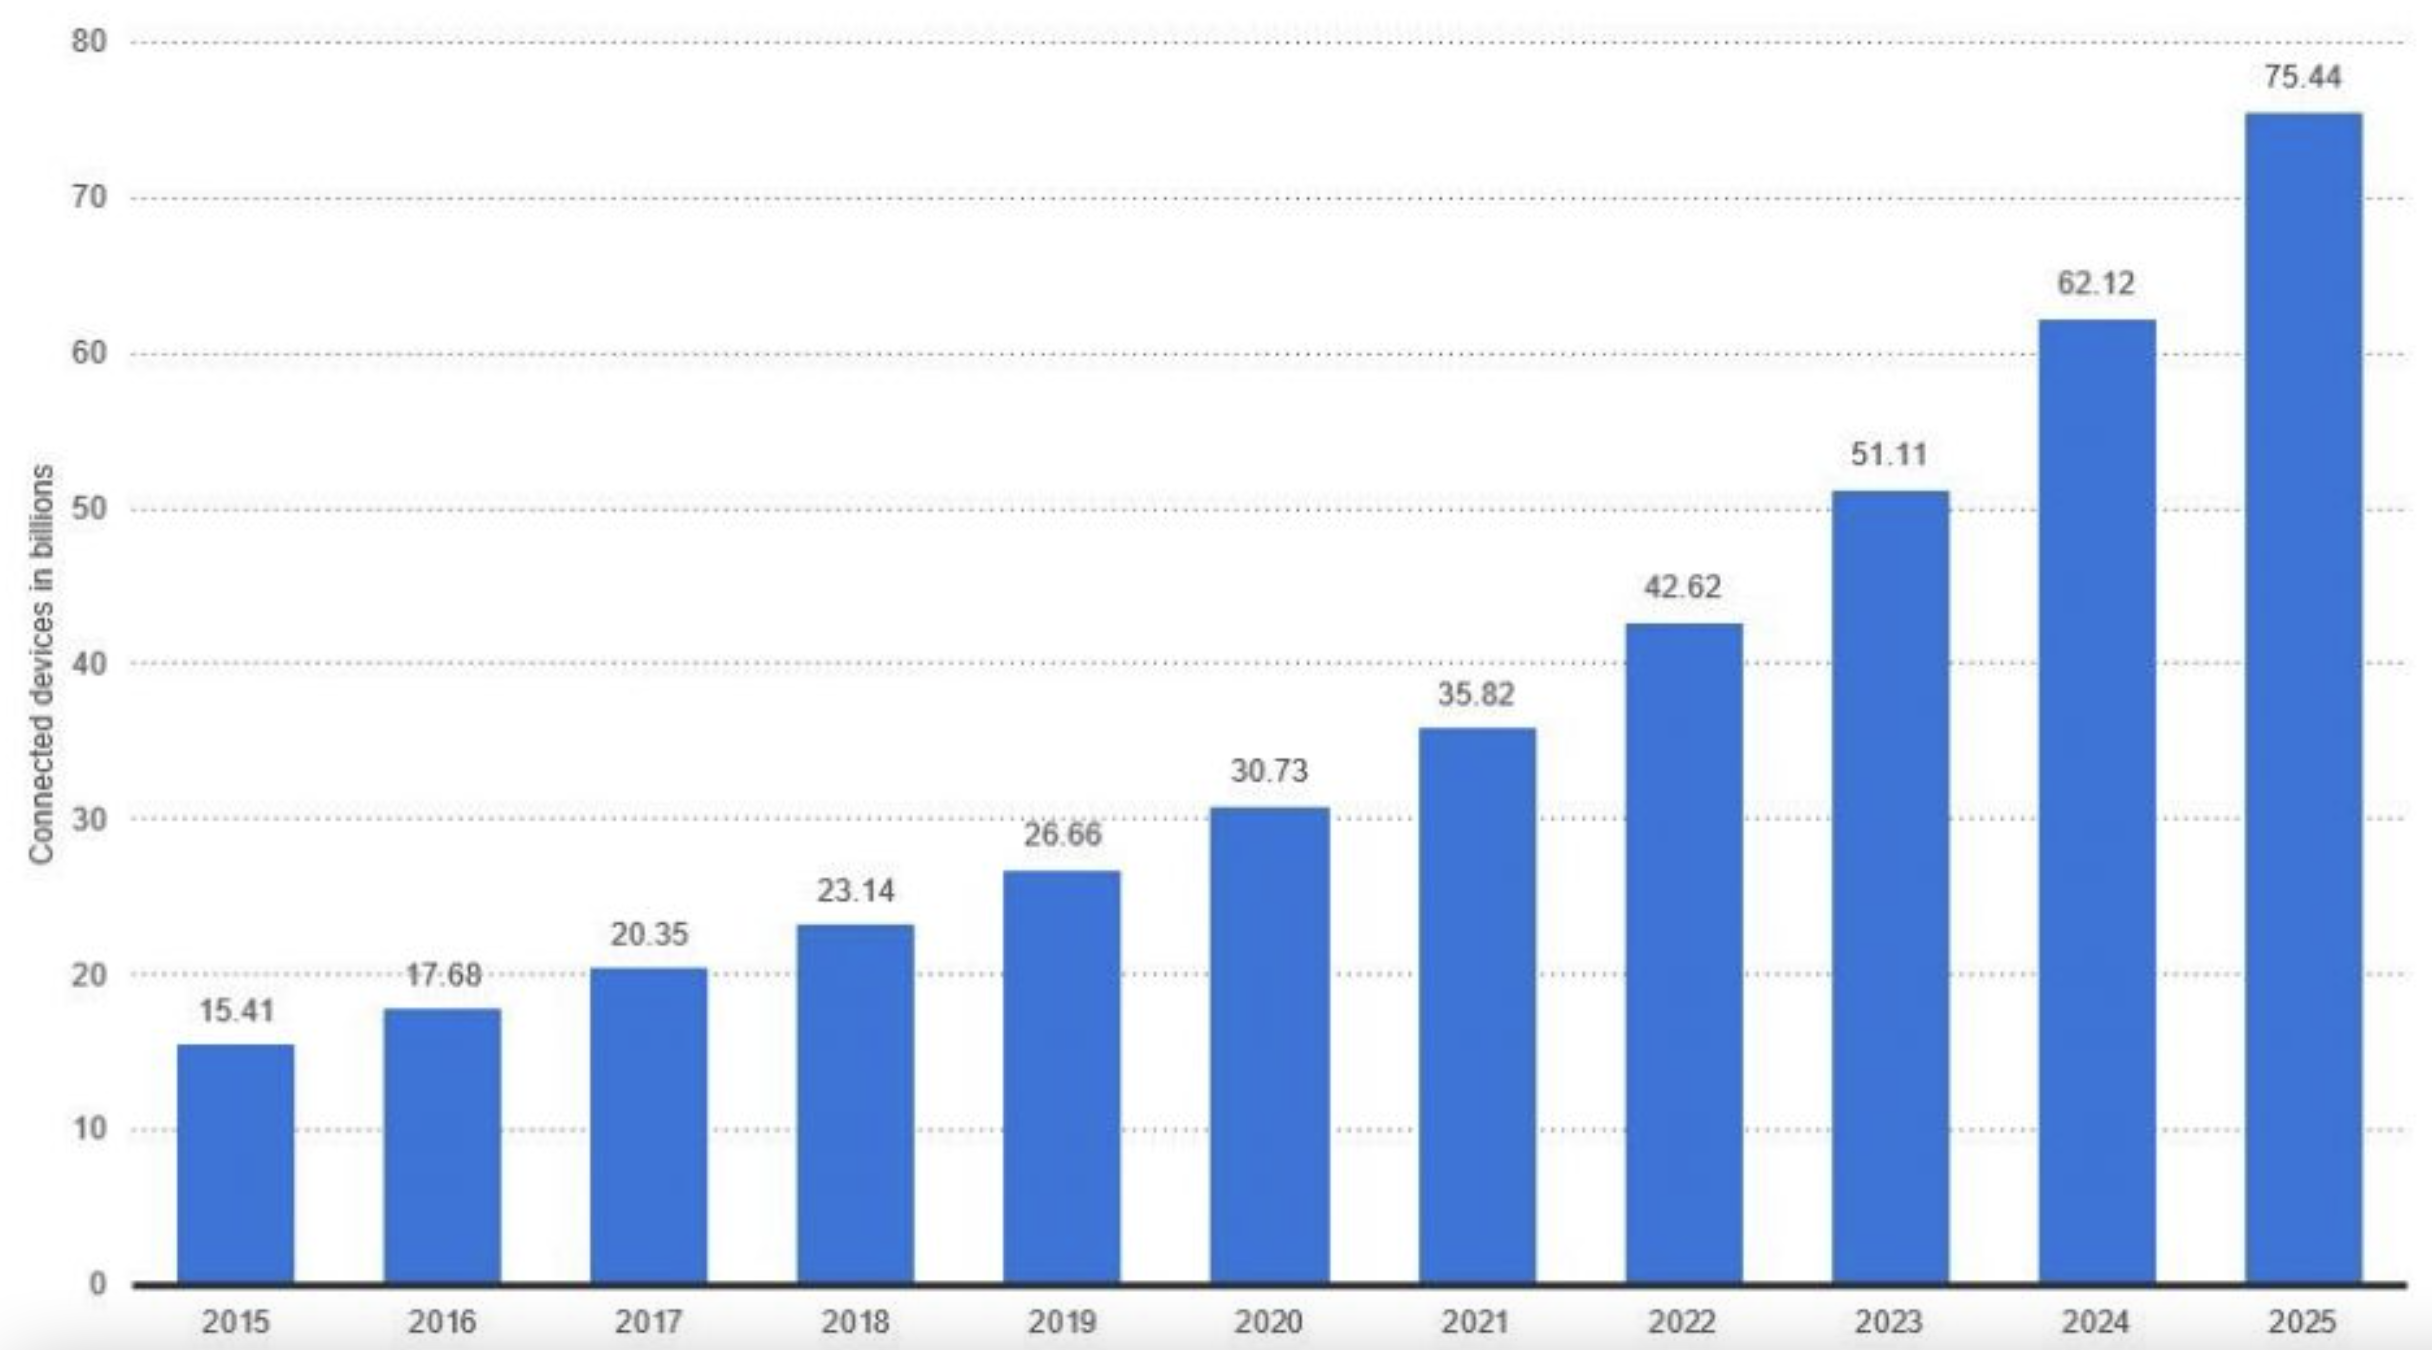
\includegraphics[scale=.3]{./Figures/iot-crecimiento.png}
	\caption[Crecimiento de dispositivos IoT]{Crecimiento exponencial de dispositivos conectados en el mundo\protect\footnotemark.}
	\label{fig:iot-crecimiento}
\end{figure}

\footnotetext{\url{https://www.iotworldonline.es/las-grandes-estadísticas-del-internet-de-las-cosas-iot/}}

%----------------------------------------------------------------------------------------

%\section{IEstado del arte}

%----------------------------------------------------------------------------------------
\section{Estado del arte}
\label{sec:estado-arte}
En la actualidad existen varias plataformas \textit{cloud} que brindan un conjunto de servicios de computación en la nube para hacer frente a las necesidades del negocio en lo que respecta al desarrollo de aplicaciones, almacenamiento y cómputo. 

Algunas de las que se encuentran consolidadas a nivel mundial son: Google, Microsoft, Amazon, Samsung, entre otras \citep{WEBSITE:6}.  Estos sistemas, si bien tienen toda la infraestructura realizada para conectar dispositivos IoT, requieren de desarrollo web que implica la programación de toda la estructura de la información que se requiere enviar a la nube.  Por otro lado,  no todas las empresas implementan como protocolo de aplicación a MQTT \citep{WEBSITE:7}.  Se resumen algunos servicios ofrecidos por estas empresas en la tabla \ref{tab:cloud-emp}.

\begin{table}[h]
	\centering
	\caption[Comparación de servicios cloud en el mercado.]{Comparación de servicios cloud en el mercado.}
	\begin{tabular}{l c c c}    
		\toprule
		\textbf{Empresa} 	 & \textbf{Servicios} 		& \textbf{Protocolo}     & \textbf{Sistema}\\
		 	 						 & \textbf{Cloud} 		& \textbf{de aplicación}     & \textbf{operativo}\\
		\midrule
		Google 			& Google Cloud 				& Weave 		& Linux\\		
		Amazon	 	& AWS IoT						& MQTT		& Linux\\
		Microsoft	 	& Azure IoT						& AMQP 		& Windows IoT\\
		Samsung	 	& SmartThings					& MQTT 		& Linux\\
		\bottomrule
		\hline
	\end{tabular}
	\label{tab:cloud-emp}
\end{table}

En cuanto a plataformas que ofrecen la etapa de procesamiento, análisis y visualización de datos, se pueden mencionar algunas como ThingBoard, Ubidots, NodeRed, entre otras. Estas plataformas asumen que el cliente cuenta con el hardware necesario para enviarles la información relevante, y ellas se encargan de analizarla y presentarla de manera conveniente mediante tableros o dashboards, que le permiten al usuario ver el estado e históricos de sensores, actuadores y nodos. 

Las principales desventajas de estas plataformas son la fuerte dependencia que generan y la poca adaptabilidad al hardware que se requiere gestionar, además, la mayoría de ellas brindan servicios con costos monetarios elevados.

%----------------------------------------------------------------------------------------

%\section{Motivacion}

%----------------------------------------------------------------------------------------
\section{Motivación}

En la actualidad existen múltiples dispositivos conversores de protocolos que permiten enviar datos a la nube, pero la mayoría no posee un sistema de gestión a través de una plataforma web. La metodología de conexión es a través de la vinculación con servicios web como los mencionados en la sección \ref{sec:estado-arte} donde el usuario deberá encargarse de realizar todo el desarrollo de la visualización de datos en forma clara, el almacenamiento de datos en una base de datos y la generación de eventos que puedan serle útil. 

Empresas multinacionales como ser ABB, Scheider Electric, Honeywell o Siemens poseen sus propias plataformas web de gestión y protocolos de comunicación, lo que genera un sistema cerrado y dependiente de un determinado fabricante de dispositivos. Por lo antes mencionado, se hace inviable la conexión de conversores de otras marcas. 

Por estos motivos, surgió la posibilidad de ofrecer un servicio de gestión web. Que contenga todos los componentes necesarios para que el usuario solo requiera de una configuración básica de conexión al servidor.  Que pueda visualizar los datos requeridos de forma remota, pudiendo generar reportes y almacenamiento de datos en breves periodos de tiempo de utilización. 

%----------------------------------------------------------------------------------------

%\section{Alcances y objetivos}

%----------------------------------------------------------------------------------------
\section{Alcances y objetivos}

\subsection{Objetivos}

El propósito de este trabajo fué el desarrollo de un sistema que contenga un servidor MQTT, una base de datos para alojar información de reportes de dispositivos y una plataforma web que permita visualizar de forma remota datos enviados de diferentes sensores que contengan instalado un conversor de protocolo Modbus a MQTT.  Esto permite maximizar la eficiencia del proceso, ya que puede ser monitoreado en tiempo real desde cualquier parte del mundo, contando con avisos de alarmas, reportes históricos y almacenamiento de datos. 

\subsection{Alcance}

Para la realización de este trabajo se propuso desarrollar una plataforma web operativa de un sistema de gestión para conversores de protocolo Modbus a MQTT que se conectan a sensores de temperatura fabricados por la empresa D\&T \citep{WEBSITE:8}.  El presente desarrollo incluye los siguientes aspectos:

\begin{itemize}
	\item Implementación de servidor MQTT.
	\item Implementación de servidor para gestión de usuarios y dispositivos.
	\item Implementación de base de datos no relacional. 
	\item Visualización de datos en tiempo real en una plataforma web. 
	\item Lectura de datos provenientes de sensores de temperatura que contenga un conversor de protocolo Modbus a MQTT.
\end{itemize}
